%--
%-- Diagrama de Contexto
%--
\subsection{Diagrama de Contexto}

%--
%-- Listado de Fenómenos
%--
\subsubsection{Listado de Fenómenos}
\begin{enumerate}

  \item Registrar cliente

  \item Iniciar sesión de usuario (puede ser cliente o admin).

  \item Cerrar sesión de usuario.

  \item Registrar pedido

  \begin{enumerate}

    \item Un cliente inicia la solicitud de un pedido

    \item Una sucursal inicia la solicitud de un pedido de reposición de
    stock

  \end{enumerate}

  \item Acordar fecha y lugar de envío

  \begin{enumerate}

    \item El website ofrece un rango de fechas para la entrega

    \item El cliente elige tres fecha de entrega

  \end{enumerate}

  \item Modificar pedido

  \begin{enumerate}

    \item Un cliente modifica un pedido

    \begin{enumerate}

      \item El Website le dá al Cliente un crédito por el valor de dicha
      mercadería (si se quita algo pago)

      \item Pagar diferencia si se agrega.

    \end{enumerate}

    \item Una sucursal modifica un pedido

  \end{enumerate}

  \item Pagar pedido

  \begin{itemize}

    \item Website entrega el crédito al Cliente si corresponde

    \item Cliente paga a Agente de Cobro (online)

    \item Agente de cobro confirma compra a website

    \item El website confirma la recepción del pago al cliente

    \item Pagar contra entrega

    \item El cliente confirma el pedido

  \end{itemize}

  \item Preparar pedido y cerrar pedido

  \begin{itemize}

    \item El website avisa al depósito que prepare el pedido

    \item Depósito informa a Depto de Stock egreso de mercadería

    \item Depósito avisa al website que el pedido está cerrado

  \end{itemize}

  \item Hacer envío

  \begin{itemize}

    \item Depósito entrega mercadería a Logística

    \item Logística entrega mercadería a Cliente (las tres fechas elegidas,
    hasta que el cliente la toma)

    \item Logística entrega la mercadería a las Sucursales

  \end{itemize}

  \item Cliente recibe pedido

  \begin{itemize}

    \item Si cliente debe dinero, paga a Logística

    \begin{itemize}

      \item Logística le devuelve el dinero a Depto de Stock
      \fixme[No tiene que devolver al departamento de stock]

    \end{itemize}

    \item Logística confirma entrega de pedido a Depósito

    \item Depósito actualiza estado de pedido a Website

  \end{itemize}

  \item Cliente no recibe pedido

  \begin{itemize}

    \item Logística devuelve mercadería a Depósito (si en ninguna de las
    fechas el cliente recibió el pedido)

    \item Depósito actualiza estado de pedido a Website

    \item Website le da un crédito al Cliente y cancela su pedido anterior

  \end{itemize}

  \item Reposición de stock de sucursal

  \begin{itemize}

    \item Una sucursal realiza un pedido al website

    \item website informa faltante de stock a Depósito

    \item Depósito entrega mercadería a Logística

    \item Logística entrega mercadería a Sucursal

  \end{itemize}

  \item Reposición de stock de Depósito

  \begin{itemize}

    \item Depto de stock recibe alarma de stock bajo 
    \fixme[enviada por el website?]

    \item Depto de stock realiza un pedido a la Proveedora correspondiente

    \item La Proveedora entrega mercadería a Logística

    \item Logística entrega mercadería a Depósito

    \item Depósito informa de ingreso de mercadería al website

  \end{itemize}

  \item Administrador consulta estadísticas al website

\end{enumerate}

%--
%-- Agentes
%--
\subsubsection{Agentes}

\begin{enumerate}
  \item Depósito
  \item Cliente
  \item Sucursal
  \item Website
  \item Logística
  \item Departamento de stock 
  \item Proveedora
  \item Agente de Cobro
  \item Administrador
\end{enumerate}

%--
%-- Acciones Básicas
%--
\subsubsection{Diagrama de Contexto: Acciones básicas}
\begin{figure}[H]
  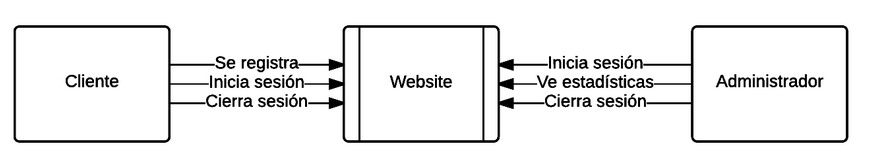
\includegraphics[width=\linewidth]{images/acciones-basicas.png}
\end{figure}
\fixme[Agregar el texto que describe este gráfico]

%--
%-- Cliente recibe pedido
%--
\clearpage
\subsubsection{Diagrama de Contexto: Cliente recibe pedido}
\begin{figure}[H]
  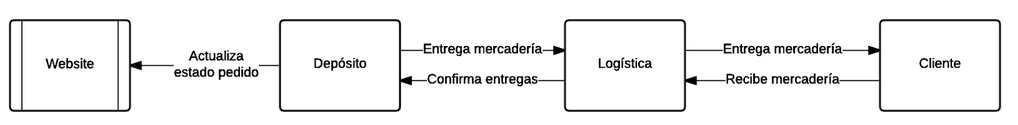
\includegraphics[width=\linewidth]{images/cliente-recibe-pedido.png}
\end{figure}
\fixme[Agregar el texto que describe este gráfico]

%--
%-- Cliente no recibe pedido
%--
\clearpage
\subsubsection{Diagrama de Contexto: Cliente no recibe pedido}
\begin{figure}[H]
  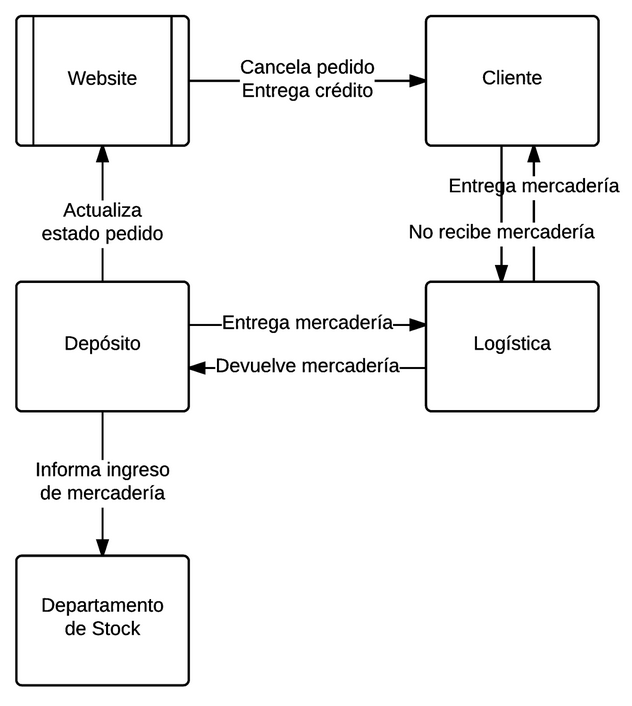
\includegraphics[width=\linewidth]{images/cliente-no-recibe-pedido.png}
\end{figure}
\fixme[Agregar el texto que describe este gráfico]

%--
%-- Reposición de stock en depósito
%--
\clearpage
\subsubsection{Diagrama de Contexto: Reposición de stock en depósito}
\begin{figure}[H]
  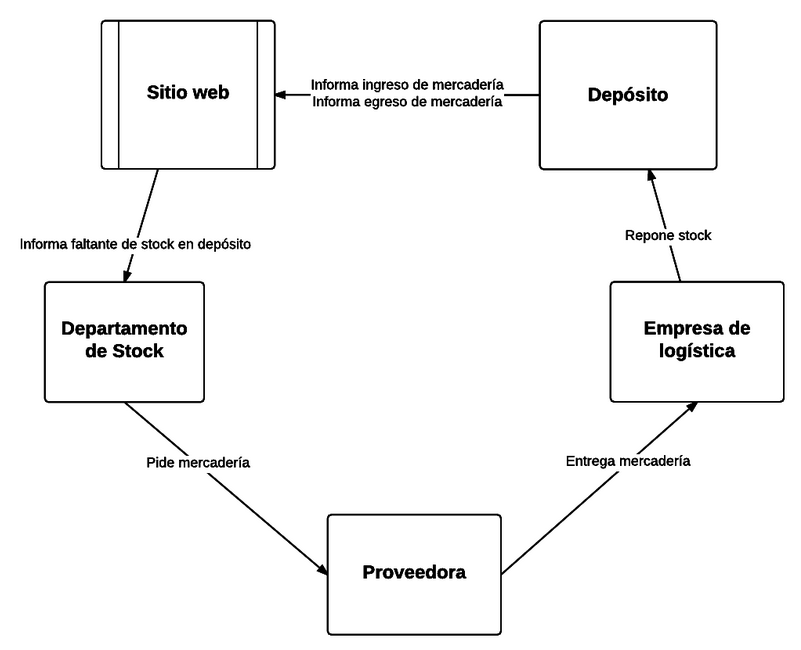
\includegraphics[width=\linewidth]{images/reposicion-stock-deposito.png}
\end{figure}
\fixme[Agregar el texto que describe este gráfico]

%--
%-- Reposición de stock en sucursal
%--
\clearpage
\subsubsection{Diagrama de Contexto: Reposición de stock en sucursal}
\begin{figure}[H]
  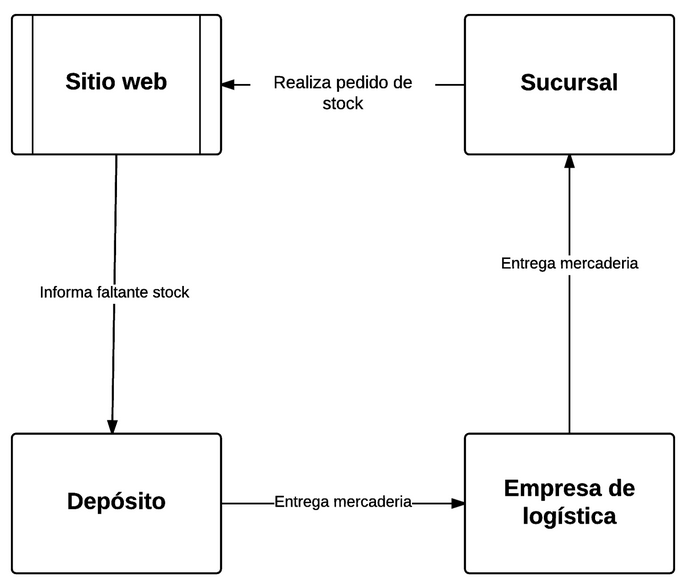
\includegraphics[width=\linewidth]{images/reposicion-stock-sucursal.png}
\end{figure}
\fixme[Agregar el texto que describe este gráfico]

%--
%-- Solicitud de pedido por cliente
%--
\clearpage
\subsubsection{Diagrama de Contexto: Solicitud de pedido por cliente}
\begin{figure}[H]
  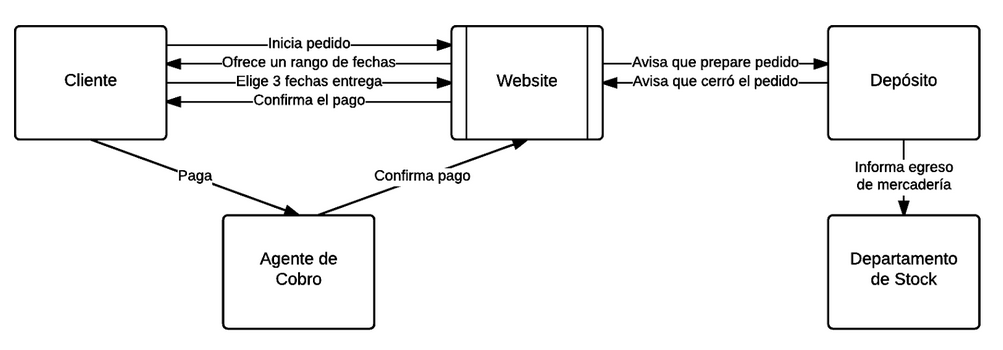
\includegraphics[width=\linewidth]{images/solicitud-de-pedido-por-cliente.png}
\end{figure}
\fixme[Agregar el texto que describe este gráfico]